
\documentclass[11pt]{article}
\usepackage{anyfontsize}
\usepackage{t1enc}

%PACKAGES%

\RequirePackage{luatex85}
\usepackage[left=0.66in, right=0.66in, top=1in, bottom=0.5in, a4paper]{geometry}
\usepackage[]{crop}
\usepackage{fontspec}
\usepackage{csquotes}%make quotes work properly for bib

\usepackage[compact]{titlesec}
\usepackage{verse}
\usepackage{letterspace}
\usepackage{sectsty}
\usepackage[hang,norule]{footmisc}
\usepackage{soulutf8}
\usepackage{enumitem}
\usepackage{supertabular}
\usepackage[usenames,dvipsnames]{xcolor}
\usepackage{placeins}%force tables to stay in place
\usepackage[hyphens]{url}
%\usepackage{makeidx}
\usepackage[tocflat, toctextentriesindented]{tocstyle}
\usepackage[unicode, hyperfootnotes=false, hyperindex=true, pdfauthor={Ajahn Brahm}, pdftitle={BSWA Divestment}, pdfsubject={Buddhism}, pdfkeywords={Buddhism}, pdfproducer={LuaTeX beta-0.70.1}, pdfcreator={LaTeX2e}]{hyperref} %ACTIVE LINKS FOR PDF AND\,ADDS METADATA%
%PACKAGES%
\hypersetup{colorlinks=true,urlcolor=MidnightBlue}

\usepackage{float}
\usepackage[printwatermark]{xwatermark}


\usepackage{graphicx}

\usepackage{draftwatermark}
\renewcommand{\figurename}{Source:}
\setlist[itemize]{noitemsep}
\setlist[enumerate]{noitemsep}

%ADD\,BLANK PAGES AT\,END\,OF BOOK%
\newcommand{\blankpage}{
\newpage
\thispagestyle{empty}
\mbox{}
\newpage
}
%ADD\,BLANK PAGES AT\,END\,OF BOOK%

%GRID%
%\usepackage{pagegrid}
%\pagegridsetup{top-left, step=1in}
%GRID%

%LINESPACE%
\usepackage{setspace}
\setstretch{1.1}
\setlength{\parskip}{0pt}
%LINESPACE%

%TABLE OF CONTENTS%
%NOTE: STYLING OF TOC IS DONE WITH TOCSTYLE. CONTROL MARGINS OF TOC BY PLACING \NEWGEOMETRY AND\,\\textsc{re}STO\textsc{re}GEOMETRY AROUND\,TOC
\settocstylefeature[]{leaders}{\hfill}%ELIMINATES DOTS%
\settocstylefeature[0]{entryvskip}{0.9em}%VERTICAL SPACE BEFO\textsc{re}\,CHAPTER ENTRIES%

\settocstylefeature[2]{entryhook}{\itshape\hspace{2.5em}}%INDENTS SUBSECTION\,ENTRIES%
\settocstylefeature[0]{pagenumberhook}{\hspace{-1em}}%COR\textsc{re}CTLY ALIGNS PAGE NUMBERS FOR CHAPTERS%
%TABLE OF CONTENTS%

%MICROTYPOGRAPHY%
\usepackage{microtype}
\frenchspacing
%MICROTYPOGRAPHY%


%HEADINGS%
\titleformat{\chapter}[display]
{\filcenter}
{\large\headcapsfont\MakeLowercase{\caps{\chaptertitlename} \thechapter}}
{1ex}
{\LARGE\itshape}



\newfontfamily\Secfont{Source Sans Pro}
\newfontfamily\Subsecfont{Literata}
\newfontfamily\Subsubsecfont{Literata}

\sectionfont{\Secfont\mdseries}
\subsectionfont{\itshape}
\subsubsectionfont{\Subsubsecfont\itshape}

%HEADINGS%


\renewcommand*{\footnotelayout}{\scriptsize\sffamily}

%FONTS%
\setmainfont[Numbers=OldStyle]{Source Serif Pro}
\setsansfont[Numbers=OldStyle]{Source Sans Pro}
\setmonofont{Source Sans Pro}

\usepackage{realscripts}
%FONTS%

%SUMMARY%

\newenvironment{summary}
{\list{}{\rightmargin \leftmargin \small \itshape}%
\item\relax}
{\endlist}

%SUMMARY%

%HANGING LEFT%
\newcommand*{\vleftofline}[1]{\leavevmode\llap{#1}}
%HANGINGLEFT%

%WIDOWS \& ORPHANS%
\widowpenalty=10000
\clubpenalty=10000
%WIDOWS \& ORPHANS%


%\brokenpenalty10000\relax

\begin{document}



\pagestyle{empty}

\subsection*{A proposal: why BSWA should put its money in ethical banking}

Due to ethical concerns, especially with fossil fuel investment, we propose that the BSWA transition its investments from Bankwest to a bank that does not invest in fossil fuels.

Fossil fuel divestment is a statement of values, withdrawing funds from companies that invest in fossil fuels. It declares that we refuse to profit from activities that cause global warming and all the harm that it brings. Globally, religious organizations have been leaders in divestment, putting morality over profit.

\bigskip

\begin{figure}[h]
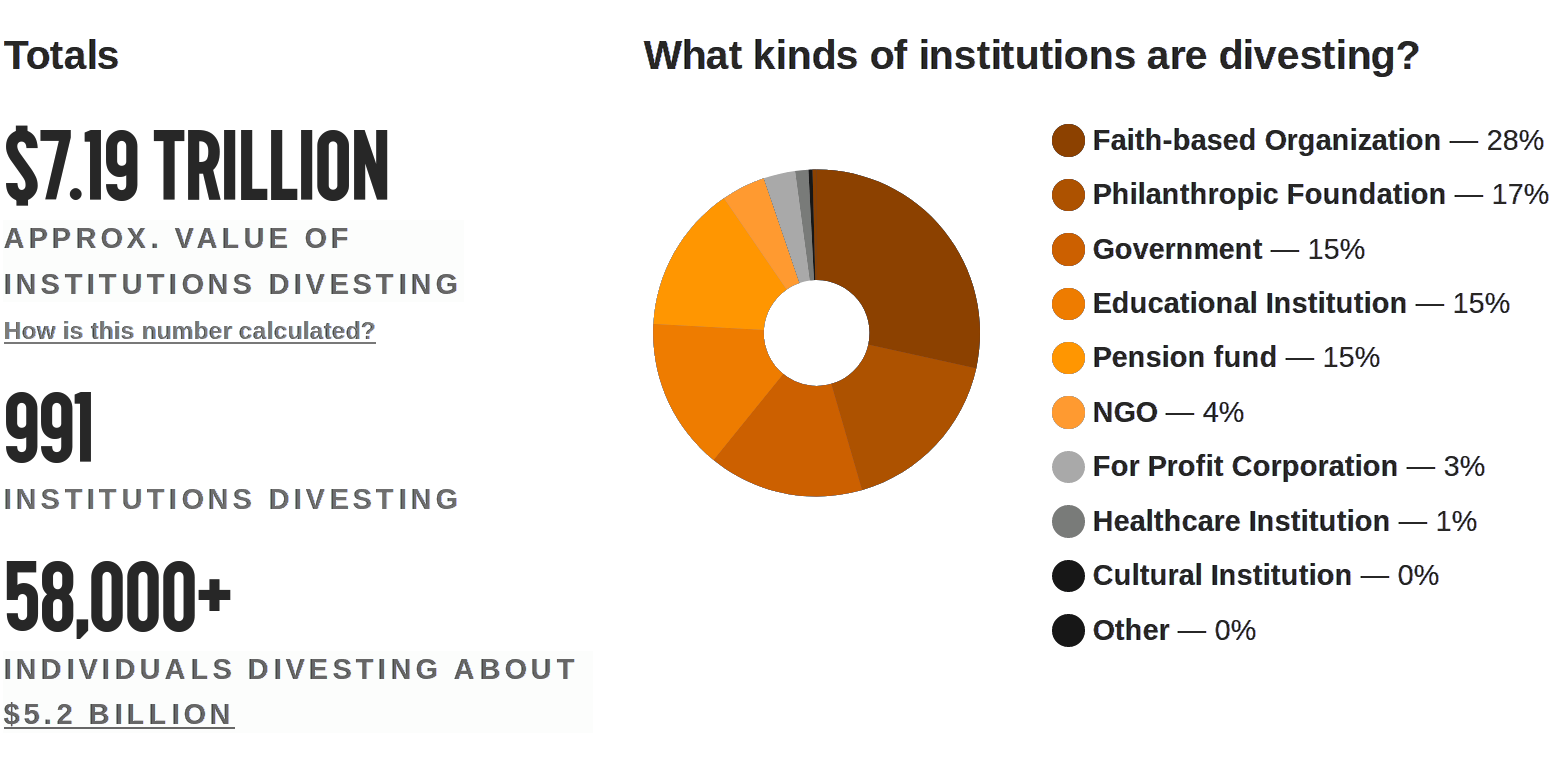
\includegraphics[width=15.9cm]{divestment.png}\\
\sffamily\scriptsize{Source: \url{https://gofossilfree.org/divestment/commitments}}
\end{figure}

\subsection*{Bankwest compared to Bendigo, a leading ethical bank}

Bankwest is owned by the Commonwealth Bank, which has loaned over \$26 billion to fossil fuels since 2008.\footnote{\url{https://marketforces.org.au/info/compare-bank-table}} That’s \$13 to fossil fuels for every \$1 to renewable energy, the worst ratio of the Big Four banks.\footnote{\url{https://marketforces.org.au/revealed-billions-loaned-to-fossil-fuels-by-the-big-banks}}

Bendigo Bank does not invest in any coal and gas projects.\footnote{\url{https://marketforces.org.au/info/compare-bank-table}} It is Australia’s fifth largest bank, with a solid credit rating \footnote{\url{https://bendigoadelaide.com.au/public/shareholders/credit\_rating/credit\_rating.asp}} and competitive term deposit interest rates.\footnote{\url{https://bendigobank.com.au/public/personal/term-deposits\#tab-335821}} It has a strong long-term policy of support for sustainability and community.\footnote{\url{https://bendigoadelaide.com.au/public/in\_the\_community/sustainable\_communities.asp}} As an example, Bendigo in Byford has contributed \$1.4 million to the local community since opening in 2008.

\subsection*{Our proposal}

The BSWA currently has significant investments in term deposits. We propose to open term deposit accounts with an ethical bank such as Bendigo as an initial step towards removing all accounts from Bankwest. We hope to show responsibility and leadership, and set an inspiring example to our members.

We ask for your support and invite your feedback.

\medskip

\noindent with metta,

\medskip

\noindent Ajahn Brahm, Bhante Sujato, Ven Pasado, Annie Keating, Boon Tan\\
\noindent October 2018



\end{document}
